\chapter{Software Parallelization Assistant}
\label{assistant}
\section{Introduction}

% problem: the need for manual parallelization, auto-parallelization does not deliver desired performance improvements

\quad Parallel hardware is ubiquitous through the entire spectrum of computing systems, from low-end embedded devices to high-end supercomputers.
%
Yet, most of the existing software is sequential.
%
Despite decades of intensive research in automatic software
parallelization~\cite{6813266}, fully exploiting the potential of modern parallel hardware still requires a significant manual effort.
%
Given the difficulty of the obstacles faced by automatic parallelization today, we do not expect that programmers will be liberated from performing manual parallelization in the near future~\cite{Larsen:2012:PML:2410141.2410600}.

% solution: parallelization assistant

This chapter introduces a novel parallelization assistant that aids a programmer in the process of parallelizing a program in the frequent case where automatic approaches fail.
%
The assistant reduces the manual effort in this process by presenting a programmer with a ranking of program loops that are most likely to 1) require little or no effort for successful parallelization and 2) improve the program's performance when parallelized.
%
Thus, it improves over the traditional, profile-guided process by also taking into account the \emph{probability} of potential parallelization for each of the profiled loops.

% how?

At the core of our parallelization assistant resides a novel machine-learning (ML) model of loop parallelizability.
%
Loops are compelling candidates for parallelization, as they are naturally decomposable and tend to capture most of the execution time in a program.
%
Furthermore, focusing on loops allows the model to leverage a large number of specific analyses available in modern compilers, such as generalized iterator recognition~\cite{Manilov:2018:GPI:3178372.3179511} and loop dependence analysis~\cite{Jensen:2017:ILD:3132652.3095754}.
%
The model encodes the results of these analyses together with basic properties of the loops as machine learning \textit{features}.

The loop parallelizability model is trained, validated, and tested on 1415 loops
from the SNU NAS Parallel Benchmarks (SNU
NPB)~\cite{Seo:2011:PCN:2357490.2358063}.
%
The loops are labelled using a combination of expert OpenMP~\cite{Dagum:1998:OIA:615255.615542}
annotations and optimization reports from Intel \cpp{} Compiler (ICC), a
production-quality parallelizing compiler.
%
The model is evaluated on multiple machine learning algorithms, including tree-based methods, support vector machines, and neural networks.
%
The evaluation shows that -- despite the limited size of the data set -- using
support vector machines allows the model to achieve a prediction accuracy higher than 90\%.
%
% Note: the "detected parallelism increase" is 945/995 - 812/995 = 0.1336683417.
%
The model improves over the ICC Compiler across the sequential C version of the SNU NPB suite by detecting 13\% more parallel loops. Albeit this improvement comes at the cost of introducing \textit{false positives}, where non-parallelizable loops are misclassified as parallelizable. However, the false positive rate in our evaluation is as low as 6.5\%. We feel this is acceptable, as our parallelization assistant does not automatically restructure code, but leaves the parallelization decision in the hands of the programmers.

The parallelization assistant combines inference on the parallelizability model
with traditional profiling to rank higher those loops with a high probability of being parallelizable and impacting the program performance.
%
An evaluation on eight programs from the SNU NPB suite shows that
the program performance tends to improve faster as loops are parallelized in the ranking order suggested by our parallelization assistant compared to a traditional order based on profiling only.
%
On average, following the order suggested by the assistant reduces by approximately 20\% the number of lines of code a programmer has to examine manually to parallelize SNU NPB to its expert-level speedup.
%
Given the high level of effort involved in manual analysis, such a reduction
can translate into substantial development cost savings.

\subsection{Motivating example}\label{motivating_example}
\quad Consider the sequential C implementation of the \textit{Conjugate Gradient (CG)}
benchmark from the SNU NPB suite.
%
Table~\ref{tab:ranking} shows the top three CG loops as ranked by the Intel
Profiler (based on their execution time) and by our parallelization
assistant (additionally taking into account their parallelizability).
%
The ranked loops compose the same loop nest with \texttt{cg.c:296} being the outermost loop and the loop \texttt{cg.c:458} being the innermost. The profiler ranks their execution time in the nesting order, while our assistant highlights the same loop nest, but, crucially, the loops are \textbf{ranked in a different order} with the innermost \texttt{cg.c:458} coming first.
\begin{table}
  \begin{minipage}{\columnwidth}
  \begin{center}
    \begin{tabu}{c|c|cc}
      \hline
      \rowfont{\bfseries}
      \multirow{2}{*}{Ranking} & Profiler & \multicolumn{2}{c}{Assistant} \\ \cline{2-4}
      \rowfont{\bfseries}
      & loop & loop & parallelizability\\\hline
      1 & \texttt{cg.c:296} & \textbf{\texttt{cg.c:458}} & 85\%\\
      2 & \texttt{cg.c:445} & \texttt{cg.c:296} & 29\%\\
      3 & \textbf{\texttt{cg.c:458}} & \texttt{cg.c:445} & 8\%\\\hline
    \end{tabu}
    \caption{Comparison of the profiler and assistant rankings for the CG benchmark loops (limited to the top three loops).}
    \label{tab:ranking}
  \end{center}
  \end{minipage}
\end{table}%
Following the profiler ranking (second column in Table~\ref{tab:ranking}), a
parallelization expert would concentrate on analyzing the longest running outermost loop \texttt{cg.c:296} first.
%
% Note: the 100 lines of code are counted using 'cloc code/cg-326.c'.
%
Analyzing this loop turns out to be costly (it consists of 100+ lines of code)
and unfruitful (it is not parallelizable due to inter-iteration
dependencies and side effects, see Listing~\ref{lst:main_iter}).
%
This analysis would be followed by an equally unfruitful analysis of \texttt{cg.c:445} being the middle loop in the nest.

In contrast, our parallelization assistant (two last columns in
Table~\ref{tab:ranking}) ranks the innermost loop \textbf{\texttt{cg.c:458}} before its two enclosing loops \texttt{cg.c:296} and \texttt{cg.c:445}, as it finds that the former has a
significantly higher probability of being parallelizable (see last column in
Table~\ref{tab:ranking}).
%
Following the assistant's ranking, a parallelization expert would thus
concentrate on analyzing the loop \textbf{\texttt{cg.c:458}} first.
%
Analyzing this loop is inexpensive (it consists of only six lines of code, see
Listing~\ref{lst:reduction}) and fruitful: its parallelization speeds up CG by a
factor of~2.8, which is~70\% of the speedup obtained by parallelizing the entire
benchmark.
%
Hence, following the ranking proposed by our assistant, a parallelization expert
can achieve most of the available speedup in CG in a fraction of the time
required by a traditional profile-guided parallelization process.
% Amdahl's law

\begin{figure}[t]
\begin{lstlisting}[caption={\texttt{cg.c:296}. The longest running loop in CG. The loop cannot be parallelized due to
inter-iteration dependences and side effects caused by system calls.},label={lst:main_iter},language=C]
for (it = 1; it <= NITER; it++) {
  ...
  if (timeron) timer_start(T_conj_grad);
  conj_grad(colidx,rowstr,x,z,a,p,q,r,&rnorm);
  if (timeron) timer_stop(T_conj_grad);
  ...
  printf("    %5d       %20.14E%20.13f\n", it, rnorm, zeta);
  ...
}
\end{lstlisting}
\begin{lstlisting}[caption={\textbf{\texttt{cg.c:458}}. Longest running loop in CG among those \emph{that can be parallelized}. Parallelization pragmas are also added to demonstrate its parallelization.},label={lst:reduction},language=C]
// lastrow - firstrow + 1 = NA, NA is the workload parameter (S=1400,M=7000,L=140000,...)
#pragma omp parallel for default(shared) private(j,k,suml)
for (j = 0; j < lastrow - firstrow + 1; j++) {
  suml = 0.0;
  for (k = rowstr[j]; k < rowstr[j+1]; k++) {
    suml = suml + a[k]*p[colidx[k]];
  }
  q[j] = suml;
}
\end{lstlisting}
\end{figure}

It would also be interesting to give a theoretical assessment of the possible CG parallel speedups with Amdahl's law \cite{10.1145/1465482.1465560}. The benchmark CG contains a number of parallelizable loops and some serial parts. The Intel Profiler reports that the main loop nest takes up 93\% of CG execution time and contains a number of parallelizable loops inside, but the longest-running \textbf{\texttt{cg.c:509}} takes up roughly 90\% of the total CG running time. It would be precise enough to assume, that 95\% of CG running time is spent executing parallelizable sections of the code. With 90\% of execution happening withing \textbf{\texttt{cg.c:509}}. The Amdahl's law derivation would yield the following estimate $s=\frac{20}{1+1/m+18/n}$, where m and n factors characterize the speedup of the corresponding parallel parts. On the 4 core machine, we experimented the factors in the formula would be around 4. So, the theoretical parallel speedups would be 3.5x for the whole CG benchmark and 3x for the innermost loop only. The theoretical speedup corresponds to what we observe experimentally (3.25x and 2.8x).
\subsection{Contributions of our Loop Parallelization Assistant}
\quad In summary, this chapter makes the following contributions:
%
\begin{itemize}
\renewcommand\labelitemi{$\vartriangleright$}
\renewcommand\labelitemii{$\bullet$}
\item We introduce a machine learning model, which can be used to predict the probability with which sequential C loops can be parallelized (Sections~\ref{predicting_parallel_loops} and~\ref{ml_predictive_performance});
\item we integrate profiling of execution time with our novel ML model into a parallelization assistant, which guides the user through a ranked list of loops for parallelization (Section~\ref{practical_applications}); and
\item we demonstrate that our tool and methodology increase programmer productivity by identifying parallel loop candidates better than existing state-of-the-art approaches (Section~\ref{evaluation}).
\end{itemize}

\section{Predicting parallel loops}
\label{predicting_parallel_loops}
\quad We approach the prediction of parallel loops as a \emph{supervised probabilistic machine learning classification problem}. Based on sequential reference applications and their manually parallelized counterparts, as well as Intel C/C++ Compiler's (ICC) parallelization reports, we create a data set of parallelizable and non-parallelizable loops. We extract loop features and use the data set to train a machine learning model, which links feature vectors describing the loops with their observed parallelizability. We then use the trained model as a probabilistic predictor: for each new loop, we determine its feature vector and then predict the probability of the loop being parallelizable \cite{Niculescu-Mizil:2005:PGP:1102351.1102430}. For naturally probabilistic models like trees, we directly use the computed classification probabilities (fraction of parallelizable training samples in the leaf node). For the support vector machines classifier, we use Platt scaling to derive the probabilities.

In this section, we introduce the parallelizability model, whereas Section~\ref{ml_predictive_performance} presents a standard ML performance assessment including accuracy, precision, and recall scores. Descriptions and definitions of the machine learning techniques we use can be found in \cite{James:2013:ISL:2517747}. We used the \textit{scikit-learn} library~\cite{scikit-learn} for all ML related tasks.

\subsection{Loop analysis \& Feature engineering}
\label{loop_analysis_and_features}
\quad For the purpose of machine learning, program loops are represented by numerical \textit{feature vectors}. We derive these features using standard compiler analyses operating on the Program Dependence Graph (PDG)~\cite{Ferrante:1987:PDG:24039.24041} of a loop. The PDG is a representation that captures both data and control information and is constructed using dependence analysis~\cite{Kennedy:2001:OCM:502981}. Figure \ref{fig:pdg} shows an example of a PDG for a simple loop, where SCC stands for \emph{Strongly Connected Component}.
\begin{figure}[ht]
\includegraphics[width=1.0\textwidth]{images/pdg_example.pdf}
\caption{Example of PDG of a simple loop with a cross-iteration dependency.}
\label{fig:pdg}
\end{figure}
We construct the PDG on a program's LLVM IR using standard dependence analysis \cite{Kennedy:2001:OCM:502981}. In addition, we use \textit{generalized loop iterator recognition}~\cite{Manilov:2018:GPI:3178372.3179511} to separate \textit{loop iterators} from \textit{loop payloads}. This enables us to define and extract features relating to each of those loop components. In total, we extract a set of 74 static loop features which are based on structural properties of the PDG and the types of instructions constituting it. Table \ref{tab:loop_features} summarizes these features.\newline\null
\quad Many features have simple and intuitive motivations behind them. Loop proportion features are backed up by the fact that larger loops tend to be harder to parallelize. Complex iterators include non-trivial cross-iteration transitions (e.g. linked-list update), unknown iteration numbers, etc. Payload SCCs introduce cross-iteration dependencies. Cohesion features characterize how tightly components of loops are coupled together in terms of the number of edges between them. Loop dependence features count the number of edges in different loop parts as well as their types. Loop instruction features characterize the loop's instruction mix, assigning more importance to memory reads/writes, calls and branches. Non-inlined function calls usually prevent loop parallelization. Intensive memory work (memory read/write fraction features) complicates parallelization as well.
\begin{table*}[!ht]{\linewidth}
  \tabulinesep=2pt
  \begin{minipage}{\linewidth}
  \begin{center}
    \begin{tabu}{M{3cm}M{3.0cm}M{5.0cm}}
      \hline
      \rowfont{\bfseries}
      Feature groups & Features & Description\\\hline
      \multirow{3}{*}{loop proportion} & absolute size & number of LLVM IR instructions\\%\hline
      & payload fraction & $\text{payload instructions} \, / \, \text{total loop instructions}$\\%\hline
      & proper SCCs number & number of payload SCCs with more than 1 instruction\\\hline
      loop dependencies & \multicolumn{2}{M{11cm}}{number of PDG edges for different dependence classes: read/write order (\emph{true}, \emph{anti}, \emph{output}), dependency type (\emph{register}, \emph{memory}, \emph{control}), other (\emph{cross-iteration}, etc.)}\\\hline
      \multirow{2}{*}{loop cohesion} & iterator/payload & $\frac{\text{edges between iterator}/\text{payload}}{\text{total loop edges}}$\\
        & critical/regular payload & $\frac{\text{edges between critical/regular payload}}{\text{total loop payload edges}}$\\
        \hline
      loop instruction nature & \multicolumn{2}{M{11cm}}{numbers and fractions of different parallelization critical instructions (memory loads and stores, branches, calls, etc.)}\\\hline
      \end{tabu}
  \end{center}
  \caption{Static features used for the characterization of loops.}
  \label{tab:loop_features}
  \end{minipage}
\end{table*}%
\subsection{Feature extraction}
\label{feature_extraction}
\quad To extract all devised loop features from SNU NPB benchmarks and get the train/test data sets we developed a tool based on the LLVM compiler infrastructure \cite{llvm-compiler-infrastructure}\cite{Lattner:2004:LCF:977395.977673}. The tool is a set of LLVM function passes working on the SSA-based LLVM IR and can be found on GitHub \cite{assistant-repo}. The tool works by building data, memory, and control dependence graphs (DDG, MDG, CDG) and combining them into the final program dependence graph (PDG) \cite{Ferrante:1987:PDG:24039.24041} for all loops found in program functions. Once all graphs are built we run the search of SCCs \cite{Manilov:2018:GPI:3178372.3179511} on them and recognise loop iterators. The final step is to traverse all these graphs computing devised metrics (ML features) and dump all that information into the file to be later fed into scikit-learn based ML scripts.
\subsection{Feature selection}
\label{feature_selection}
\quad The feature engineering task produced a quantitative description of program loops being characterised by feature vectors of length 74. To avoid overfitting, we discard irrelevant or redundant features using a pipeline of automatic feature selection methods from the scikit-learn library. First, we eliminate features with a low variance score, then we fit a decision tree-based model and select features with importance scores above a given threshold. After that, we repeatedly run \textit{Recursive Feature Elimination, Cross-Validated (RFECV)} to improve accuracy, precision, and recall scores. This yields the final set of features. Table \ref{tab:best_features} presents the 10 highest-ranked features in the set. SNU NPB benchmarks contain a lot of uninlined function calls and, unsurprisingly, the amount of call instructions in the payload of a loop ranks the highest. Despite the absence of straightforward intuition behind cohesion metrics, they tend to correlate with loop parallelizability well. Loops heavy on memory writes also significantly affect the parallelizability property.
\begin{table}[ht]
  \begin{minipage}{\columnwidth}
  \begin{center}
    \begin{tabu}{lc}
      \hline
      \rowfont{\bfseries}
      \multicolumn{1}{l}{Feature} & \multicolumn{1}{l}{Importance}\\\hline
      payload call fraction & 23.5\\
      iter/payload non-cf cohesion & 18.5\\
      payload mem write fraction & 6.1\\
      loop absolute size & 5.7\\
      critical payload pointer access count & 5.3\\
      payload memory dependence count & 4.0\\
      critical payload non-cf cohesion & 2.9\\
      payload pointer access fraction & 2.7\\
      critical payload total cohesion & 2.6\\\hline
      \end{tabu}
  \end{center}
  \end{minipage}
  \caption{Relative importance of static loop features, ranked by fitting a tree-based ML model.}
  \label{tab:best_features}
\end{table}
\subsection{Model \& Hyper-parameter selection}
\label{model_selection}
\quad We evaluate several machine learning classification algorithms in our parallelization assistant, including tree-based methods like decision trees (DT), random forests (RFC), and boosted decision trees (AdaBoost); support vector machine classifiers (SVC) and multi-layer perceptron neural networks (MLP). Section \ref{evaluation_kfold} shows that these models perform similarly with SVC and MLP performing slightly better. For each ML model, we use exhaustive hyper-parameter grid search and pick the grid node with the best cross-validation score on the validation set. The details of all ML pipeline stages are available in our repository \cite{assistant-repo}.
\subsection{Training data \& ML model training}
\label{loop_classification_labels}
\quad In order to train and test our ML model in a supervised way, first we need to provide it with the "right answers" regarding loop parallelizability. In other words, we need to prepare a labelled training data set. For training our ML model we use a total of 1415 loops from the SNU NPB benchmark suite. Out of those loops, 210 have been annotated by (external) human experts with parallel OpenMP \textit{pragmas}. Like \cite{fried_ea:2013:icmla} we use these annotations as labelled data to indicate parallelizable loops. However, the data is not complete. Human programmers strive to capture only coarse-grain parallelism and do not annotate every parallelizable loop. Hence, we augment the training data with the help of the ICC Compiler, which finds additional parallelizable loops. We combine the results into our final training set comprising a total 1415 loops, of which 995 are labelled as parallelizable. Then we use K-fold and Leave-One-Out Cross-Validation (LOOCV) methodologies to train and test our ML models.\newline\null
\quad To extract loop parallelizability labels from the Intel compiler's optimization reports we developed a parser \cite{github-icc-parser}, but the task has presented us with a number of technical challenges. Before ICC can actually parallelize or vectorize a loop, it applies a number of enabling loop transformations such as loop interchange, distribution, tiling, etc. These transformations help ICC to eventually uncover more parallelism. The detailed description of all these transformations can be found in \cite{Bacon:1994:CTH:197405.197406}. Applied to a loop nest, these optimizations might significantly restructure and distribute the parts of a loop across the whole ICC optimization report. Moreover, ICC might parallelize only certain parts of transformed loop. In the end, we considered a loop to be parallelizable by the ICC compiler if the latter hasn't found any dependencies and either vectorized or parallelized it. In the case of distributed loops, all parts must be parallelizable for an original loop to be considered as such. For a final correctness we conducted a manual verification on top of automatically extracted results.\newline\null
\quad Table \ref{tab:icc_stats} presents a parsing report, which summarises the number of times ICC applied a certain optimization. The major cells are \textit{parallel} and \textit{icc}, which report the total number of truly parallelizable loops and the number of loops parallelized by ICC. As can be seen, ICC compiler does not exploit all the parallelism available in SNU NPB benchmarks. Section \ref{background_challenges_automatic} presented a study of the reasons why ICC fails to parallelize certain loops. To obtain the data we used ICC 18.0. As we are interested in obtaining the most complete set of parallelization labels, and not in the optimal program running time, we instructed ICC to do the most aggressive parallelization, i.e. parallelize a loop, whenever it can be parallelized, ignoring ICC cost model and independent of the expected profitability of loop parallelization (\textit{-parallel -vector -par-threshold0} options). To make ICC uncover all possible parallelism we ran it with a wide set of enabling loop transformations (\textit{-O3} option) applied prior to the parallelization. All the options had a matching hardware support: we installed ICC on the Ubuntu 18.04 machine with 4 Intel Core i5-6500 CPUs having a vectorization support all up to AVX2.
\begin{table}
  \begin{minipage}{\columnwidth}
  \begin{center}
    \begin{tabu}{cccccc}
      \hline
      \rowfont{\bfseries}
      \multicolumn{2}{c}{\multirow{2}{*}{Labels}} & \multicolumn{4}{c}{Intel Compiler (ICC)} \\%\hline
      \rowfont{\bfseries}
      & & \multicolumn{2}{c}{Optimization} & \multicolumn{2}{c}{Parallelization}\\\hline
      loop & ranking & loop & ranking & parallel \\\hline
      \textbf{total loops} & \textbf{1415} & distrs & 34 & parallel & 653\\
      \textbf{parallel} & \textbf{995} & fusions & 214 & vector & 737\\
      \textbf{icc} & \textbf{812} & collapses & 58 & parallel deps & 535\\
      \textbf{openmp} & \textbf{210} & tilings & 27 & vector deps & 266\\\hline
    \end{tabu}
  \end{center}
  \end{minipage}
  \caption{Report on loop classification labels derived from expertly added OpenMP annotations of SNU NPB benchmarks and ICC optimization reports. Out of all 995 parallelizable loops the ICC discovered and parallelized only 812.}
  \label{tab:icc_stats}
\end{table}
\section{ML predictive performance}
\label{ml_predictive_performance}
\quad In our work we employ 2 cross-validation (CV) techniques. We evaluate the overall predictive performance our trained ML model is capable of achieving on SNU NPB benchmarks using K-fold CV. To deploy our assistant against single benchmarks of the suite and assess its effectiveness (Section \ref{evaluation}) we have to use a modified Leave-One-Out CV.
\subsection{Overall model performance}
\label{evaluation_kfold}
\quad Table \ref{tab:average_accuracy_models} shows the overall predictive performance of different ML models measured with K-fold CV on the whole SNU NPB data set. Training and testing have been done for different values of K (5, 10, 15, 20, 25, 30) and the accuracy remains stable across the entire range. The same is true of recall and precision scores. We used the baselines (constant "parallelizable" prediction and uniform) available in scikit-learn to compare our models against.
\begin{table}
  \begin{minipage}{\columnwidth}
  \begin{center}
    \begin{tabu}{cccc}
      \hline
      \rowfont{\bfseries}
      ML model & accuracy & recall & precision\\\hline
      constant & 70.32 & 100 & 70.32\\
      uniform & 46.27 & 41.50 & 69.79\\
      SVC & 90.04 & 95.24 & 91.06 \\
      AdaBoost & 86.96 & 92.92 & 89.06 \\
      DT & 84.36 & 89.57 & 87.90 \\
      RFC & 86.65 & 93.22 & 88.47 \\
      MLP & 89.40 & 93.77 & 91.39 \\\hline
      \end{tabu}
  \end{center}
  \end{minipage}
  \caption{Average predictive performance of different ML models measured with K-fold CV on the whole set of 1415 SNU NPB loops.}
  \label{tab:average_accuracy_models}
  \vspace{-5mm}
\end{table}
The SVC model has the highest average accuracy and successfully manages to recall 95.24\% of all parallel loops. The ICC Compiler succeeds in parallelizing 812 out of 995 parallelizable loops available in SNU NPB. Thus, on average SVC extends the ICC Compiler's parallelization capabilities to 948 loops. Figure \ref{fig:prediction_stats} shows that out of the 10\% of mispredictions that SVC makes, 65\% are false positives. Hence, the average unsafe error rate is 6.5\%. In this project, though we devise a scheme, that protects us and makes these errors not critical.
\begin{figure}[ht]
\includegraphics[width=1.0\textwidth]{images/prediction_stats.pdf}
\caption{Breakdown of misclassification errors.}
\label{fig:prediction_stats}
\vspace{-5mm}
\end{figure}
\subsection{Model performance within assistant}
\label{evaluation_loocv}
\quad Our proposed assistant (Section \ref{practical_applications}) is trained and tested using LOOCV rather than K-fold CV. Instead of treating the entire set of loops from all SNU NPB benchmarks as a single data set, in this context, we train the model on nine benchmarks and test it on the remaining one. Doing so completely excludes the loops of the target benchmark out of a training set, but allows us to get predictions for all benchmark loops, parallelize them if advised so, and test the effectiveness of our assistant. The drawback of this scheme is that it might potentially reduce the accuracy if the nature of loops in the target benchmark dramatically differs from that of loops seen in the training set. Figure \ref{fig:accuracy_loocv_vs_kfold} compares LOOCV accuracy against that of K-Fold CV for all SNU NPB benchmarks, where K-Fold CV is conducted on a data set consisting of loops from a single benchmark only. The comparison proves that lower LOOCV accuracies are attributed to a reduced training data set and not to our ML model.
\begin{figure}[ht]
\includegraphics[width=1.0\textwidth]{images/LOOCV_accuracy.pdf}
\caption{Prediction accuracy measured with modified LOOCV and compared against that of K-fold CV for single benchmarks.}
\label{fig:accuracy_loocv_vs_kfold}
\vspace{-5mm}
\end{figure}
\section{Parallelization assistant}
\label{practical_applications}
\quad The ML-based predictor developed and assessed in the 2 previous sections can have a real practical application. Due to the statistical nature inherent to all machine learning techniques, it is impossible to eliminate all prediction errors. While false negatives might just miss available parallelization opportunities and lose some performance, false positives can break the program and are the most critical in the context of our ML problem. Given that, we develop a parallelization assistant, which does not seek to replace programmers but aims to assist and increase their productivity. The predictor is the core component of our novel parallelization assistant. The assistant incorporates prediction results and combines them with profiling information. It then produces a ranking of all loops in an application to guide a programmer towards the most beneficial loop candidates for their \textit{manual} parallelization effort.\newline\null 
\quad \textbf{Loop Ranking.} The loop ranking computed by our parallelization assistant combines a loop's contribution to the overall program execution time with its predicted probability of being parallelizable. In particular, we obtain the ranking by applying a shifted sigmoid function to the predicted probability multiplied by the application runtime fraction a loop takes to run as shown in Figure \ref{fig:sigmoid_3d}.
\begin{figure}[ht]
\includegraphics[width=0.75\textwidth]{images/product_func.pdf}
\centering
\caption{For each loop the ranking function combines its contribution to the application's execution time and its predicted probability of being parallelizable.}
\label{fig:sigmoid_3d}
\end{figure}
The intuition for using this function to combine the two metrics is that it prioritizes parallelizable long-running loops and scales down the weight of non-parallelizable loops irrespective of their contribution to execution time. The effect of this can be seen in Figure \ref{fig:ft_loop_ranking} for the loops of the FT benchmark.
\begin{figure}[htb!]
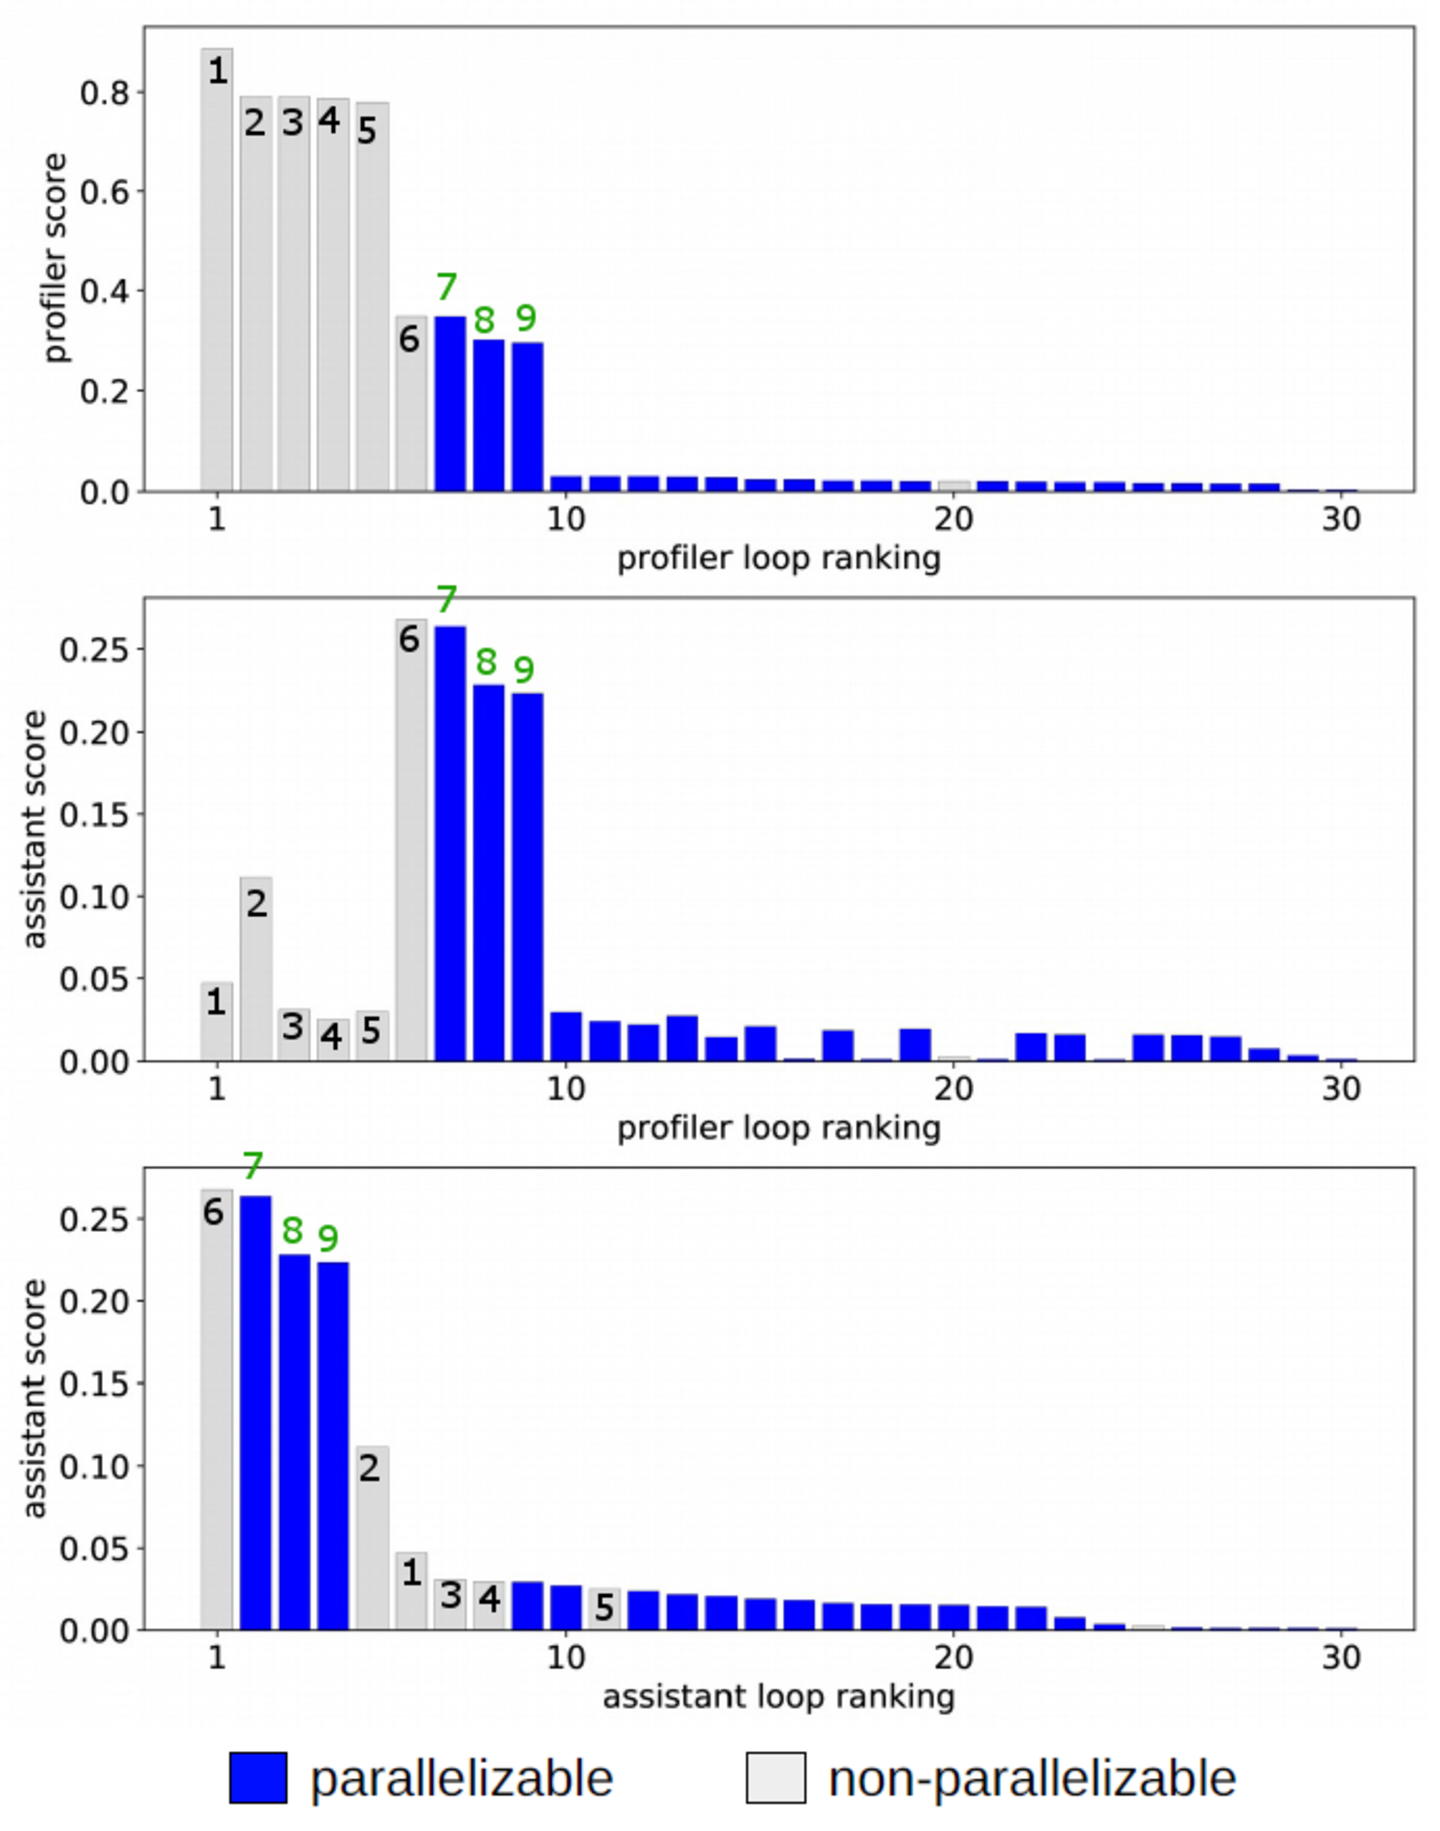
\includegraphics[width=1.0\textwidth]{images/ft_filter_nums.pdf}
\caption{Change of loop rankings with the application of the assistant ranking function for the 46 loops of the FT benchmark. Ranking based on loop execution time alone (top figure) results in some high-ranked, but non-parallelizable loops. Combining profiled execution time and parallelizability in a single score (middle figure) results in a ranking that prioritizes parallelizable loops (bottom figure).}
\label{fig:ft_loop_ranking}
\end{figure}
If programmers attempt to parallelize loops in the order prescribed by their execution time, they will inevitably waste
their efforts trying to parallelize loops that may be long-running, but offer little or no opportunity for extracting parallelism. Instead, by taking into account predicted parallelizability our ranking directly guides the programmer towards loops that significantly contribute to overall execution time \textbf{and} offer a realistic prospect of parallelization.
%Top left and right pictures are identical and rank FT benchmark loops according to their running time score (given by the Intel Compiler). The problem with that order is that it ranks long-running program loops the highest independent of their parallelisability. If a programmer starts to parallelise application following that order, he is going to waste his time and efforts on the loops one cannot parallelise anyway. The left and right plots at the bottom of the figure demonstrate a transformation in the loop ranking our assistant does. Vertical axes of these plots correspond to the values our shifted sigmoid ranking function (see figure \ref{fig:sigmoid_3d}) takes. The bottom left plot shows how the relative height of the bars changes with a switch from a loop runtime to our scoring function. It is clear from the plot, that non-parallelisable loops go down in their importance. The bottom right picture shows that such a change actually moves true parallel loops toward the beginning of the list. The longer loop takes to run, the bigger the move. On the other hand non-parallelisable loops move towards the back of the list (almost independent of their running time). The improved ranking of FT loops allows a programmer to immediately start benchmark parallelisation with the most important loops and don't waste time looking at long-running loops, which cannot be parallelised by their nature anyway.
\section{Assistant evaluation}
\label{evaluation}
\subsection{Comparison to static analysis}
\label{assistant_predictor_vs_icc}
\quad We have compared the generated loop parallelizability classifications of our assistant against that of the ICC Compiler, which due to its use of static analysis is conservative and occasionally misses some parallelization opportunities. The ML approach to parallelization with a human programmer responsible for final code transformation allows our parallelization assistant to be more aggressive than the ICC Compiler. In other words, our model can discover more parallelizable loops.\newline\null
\quad We have set up an experiment where we apply our ML predictor side-by-side with the ICC Compiler, which has been configured to do the most aggressive parallelization (see Section \ref{loop_classification_labels}) on the same machine, that provides all hardware support needed. Both, the assistant and the ICC aim at independently classifying loops as parallelizable or not. There is a total of six possible classification combinations that our scheme might produce. Figure \ref{fig:icc_competition} shows their relative distribution as a pie chart. To calculate the relative frequency of different loop classification combinations illustrated in Figure \ref{fig:icc_competition} we repeatedly ran K-fold CV on the whole set of SNU NPB loops and sorted the outcomes into separate classification buckets. In the ``agreement'' cases, which number around 80\% of cases the ICC Compiler and ML predictor identically classify truly (non-)parallelizable loops as (non-)parallelizable. This is an expected result, since we used ICC (along with OpenMP annotated loops) to train our ML model. The ``missed opportunity'' cases, where both ICC Compiler and ML predictor miss parallelizable loops also represent the agreement and are not interesting. The most interesting cases though are those, where ML predictor and the ICC Compiler disagree. While ICC Compiler is conservative and will never classify a non-parallelizible loop as parallelizible, the statistical ML predictor can make a ``false positive'' error. The rate of false positives in this experimental setting is 8\%. That works in the opposite direction as well. The ML predictor can discover truly parallelizible loops, which escape compiler analysis. The rate of such cases is 10\%. These cases are classified as ``discovery'' and have been manually checked in the source code of SNU NPB. The results are summarized in Table \ref{tab:icc_missed_opportunities}, which reports on the reasons behind ICC conservativeness. False negative mispredictions make ML predictor miss some real parallelization opportunities, but in the fraction of these cases the ICC Compiler can catch them and ``shield'' the ML predictor.
\begin{table}
  \tabulinesep=2pt
  \begin{minipage}{\columnwidth}
  \begin{center}
    \begin{tabu}{M{3cm}M{0.5cm}M{3cm}M{0.5cm}M{3cm}M{0.5cm}}
      \hline
      \rowfont{\bfseries}
      Reason & Num & Reason & Num & Reason & Num\\\hline
      missed reduction & 18 & array privatization & 7 & conservative analysis & 60\\\hline
      unknown iteration number & 7 & static dependencies & 46 & too complex & 22\\\hline
      non-inlined calls & 4 & other & 4 & total & 168\\\hline
    \end{tabu}
  \end{center}
  \end{minipage}
  \caption{Classification of parallelizable loops rejected for parallelization by the ICC Compiler. The ICC conservativeness is largely explained by the presence of pointers and limitations of alias analysis. Static dependencies are mostly created by indirect array references.}
  \label{tab:icc_missed_opportunities}
  \vspace*{-5mm}
\end{table}%
\begin{figure}[t!]
    %\begin{minipage}{\columnwidth}
    \centering
    %\includegraphics[trim=1mm 1mm 1mm 1mm,clip,width=0.9\columnwidth]{figures/icc_vs_predictor.pdf}
    \includegraphics[width=0.6\textwidth]{images/pie.pdf}
    \caption{
      Distribution of loop classifications by the ICC Compiler and our predictor.}
    \label{fig:icc_competition}
%\end{minipage}
\vspace*{-5mm}
\end{figure}
\begin{figure*}[t!]
\centering
\includegraphics[width=1.0\textwidth]{images/perf_conv_curves_new.pdf}
\caption{From left to right more loops are parallelized for each benchmark. As we parallelize more loops, program execution times improve over the initial sequential performance and reach the performance level of the reference OpenMP implementations. Our ML based parallelization assistant requires the user to parallelize fewer loops than a purely profile-guided approach to reach the maximum parallel speedup.}
\label{fig:performance_convergence_line}
\vspace*{5mm} % Just to fill up the rest of the page
\end{figure*}
\subsection{SNU NAS parallelization}
\label{assistant_snu_npb_parallelization}
\quad In this section we evaluate the effectiveness of our parallelization assistant. In particular, we are interested in the potential programmer productivity gains delivered by our tool and savings on human expert time. Our study assumes that the human expert starts with a sequential version of the SNU NPB benchmarks. The goal is to parallelize these applications to a performance level matching that of their existing parallel versions. By using our assistant we expect the human expert to consider fewer loops than by using a profiling-based approach, i.e.\ considering loops in decreasing execution time.\newline\null
\quad For this experiment we used a desktop Ubuntu 18.04 machine and compiled the benchmarks with the Intel C/C++ Compiler (ICC) 18.0. We compiled the serial versions with \textit{-O3} and \textit{-ipo} flags and explicitly prohibited any vectorization (\textit{-no-vec}) or parallelization (\textit{-no-par}). The OpenMP parallel versions have also been compiled with \textit{-O3} and \textit{-ipo} flags and prohibited automatic parallelization. When we followed the rankings and parallelized benchmarks loop by loop we used OpenMP pragmas and compiled the code with \textit{-O3} and \textit{-ipo} flags as well. Benchmark running times have been measured with the help of UNIX time() utility. To minimize the errors, we ran experiments several times and took the mean average. The machine has 4 Intel Core i5-6500 CPUs with 3.20 GHz frequency and vectorization support up to AVX2. The RAM is 16Gb.\newline\null
\quad Figure~\ref{fig:performance_convergence_line} summarizes our results as performance convergence curves. For each benchmark the curves plot its execution
time (y-axis) as a function of the number of analyzed and possibly parallelized
loops (x-axis). The runtime is bounded within the runtime of the serial
execution (top dashed line) and the time of the reference parallel OpenMP version (bottom dashed line). Our goal is to reach the performance of the reference parallel versions of each program by parallelizing them one loop at a time following the rankings offered by our assistant and the profiler. The neural network based MLP model of our assistant provides the fastest overall performance
convergence. While there is some variation depending on the ML model used for
the parallelization prediction, in general ML-assisted parallelization
outperforms or equals the profile-guided schemes across all benchmarks.\newline\null
\quad Following the rankings of our assistant in parallelizing the BT, CG and FT
benchmarks, we reach their maximum potential performance faster. For BT, maximum
parallel performance can be reached after the user has parallelized the first three loops (3061 LOC in Table \ref{tab:parallelization}) suggested by our assistant, while profile-guided parallelization requires 6 loops (6122 LOC) to be parallelized first before reaching the same performance level. For CG, if we follow the suggestion of our assistant to first parallelize a small loop (6 LOC), we are able to achieve 70\% of the maximum potential speedup (see Section~\ref{motivating_example}). On the other hand, using the profiler ranking requires examining three loops, totalling to 330 LOC, to yield the same performance gains. Moreover, for the SP and UA benchmarks, some of the assistant rankings require the programmer to examine more loops than the profiler. However, the loops proposed by the assistant in the UA benchmark are actually simpler, since they consist of fewer LOC -- 508 LOC for MLP and 579 for DT versus the 882 LOC offered by the profiler. By following our assistant's suggestions, a
programmer would be required to examine 20\% less LOC on average across all models.\newline\null
\quad In some cases, partial benchmark parallelization might result in a slowdown. In the case of LU, after having parallelized the first 25 loops we do not converge to the best achievable parallel version performance. There are a total of 40 OpenMP pragmas in the benchmark and we need to parallelize all the respective loops to reach the best performance level. In the case of UA, all rankings suggest analyzing a long-running innermost loop first. Its parallelization actually increases running time due to a synchronization barrier being introduced at a wrong program point. It takes 30 loops for the MLP model to achieve the parallel version performance.

\begin{table*}[t]
  \scriptsize
  \begin{minipage}{\textwidth}
  \begin{center}
    \begin{tabu}{c|ccc|cc|c|ccccc}
      \hline
      \rowfont{\bfseries}
      \multirow{2}{*}{Bench.} & \multicolumn{3}{c}{Bench.~Runtime, \textit{sec}} \vline & \multicolumn{2}{c}{Speedup, \textit{times}} \vline & \multicolumn{6}{c}{$Loops\ Number_{LOC}$}\\\cline{2-12}
      \rowfont{\bfseries}
      & Serial & OpenMP & Critical & OpenMP & Critical & Profile & SVC & MLP & RFC & AdaBoost & DT\\\hline
      BT & 158.76 & 57.36 & 56.57 & 2.77 & 2.81 & $6_\textit{6122}$ & \cellcolor[HTML]{FA8D8D} $8_\textit{6392}$ & \cellcolor[HTML]{7BB66B} $4_\textit{4088}$ & \cellcolor[HTML]{7BB66B} $5_\textit{5105}$ & \cellcolor[HTML]{7BB66B} $3_\textit{3061}$ & \cellcolor[HTML]{7BB66B} $5_\textit{5105}$\\
      CG & 69.38 & 19.77 & 25.06 & 3.51 & 2.77 & $3_\textit{330}$ & \cellcolor[HTML]{7BB66B} $2_\textit{118}$ & \cellcolor[HTML]{7BB66B} $1_\textit{6}$ & \cellcolor[HTML]{7BB66B} $1_\textit{6}$ & \cellcolor[HTML]{7BB66B} $1_\textit{6}$ & \cellcolor[HTML]{7BB66B} $1_\textit{6}$\\
      DC & 698.82 & 254.29 & 698.82 & 2.75 & 1.00 & $\infty$ & \cellcolor[HTML]{91A1FA} $\infty$ & \cellcolor[HTML]{91A1FA} $\infty$ & \cellcolor[HTML]{91A1FA} $\infty$ & \cellcolor[HTML]{91A1FA} $\infty$ & \cellcolor[HTML]{91A1FA} $\infty$\\
      EP & 86.35 & 35.40 & 35.07 & 2.44 & 2.46 & $1_\textit{45}$ & \cellcolor[HTML]{91A1FA} $1_\textit{45}$ & \cellcolor[HTML]{91A1FA}$1_\textit{45}$ & \cellcolor[HTML]{91A1FA} $1_\textit{45}$ & \cellcolor[HTML]{91A1FA} $1_\textit{45}$ & \cellcolor[HTML]{91A1FA} $1_\textit{45}$\\
      FT & 36.81 & 12.13 & 14.69 & 3.03 & 2.51 & $9_\textit{338}$ & \cellcolor[HTML]{7BB66B} $4_\textit{187}$ & \cellcolor[HTML]{7BB66B} $3_\textit{140}$ & \cellcolor[HTML]{7BB66B} $4_\textit{187}$ & \cellcolor[HTML]{91A1FA} $9_\textit{338}$ & \cellcolor[HTML]{7BB66B} $5_\textit{193}$\\
      IS & 4.75 & 1.35 & 4.63 & 3.53 & 1.03 & $\infty$ & \cellcolor[HTML]{91A1FA} $\infty$ & \cellcolor[HTML]{91A1FA} $\infty$ & \cellcolor[HTML]{91A1FA} $\infty$ & \cellcolor[HTML]{91A1FA} $\infty$ & \cellcolor[HTML]{91A1FA} $\infty$\\
      LU & 115.46 & 55.00 & 140.53 & 2.10 & 0.82 & $\infty$ & \cellcolor[HTML]{91A1FA} $\infty$ & \cellcolor[HTML]{91A1FA} $\infty$ & \cellcolor[HTML]{91A1FA} $\infty$ & \cellcolor[HTML]{91A1FA} $\infty$ & \cellcolor[HTML]{91A1FA} $\infty$\\
      MG & 5.20 & 3.58 & 3.94 & 1.45 & 1.32 & $3_\textit{43}$ & \cellcolor[HTML]{91A1FA} $3_\textit{43}$ & \cellcolor[HTML]{91A1FA} $3_\textit{43}$ & \cellcolor[HTML]{91A1FA} $3_\textit{43}$ & \cellcolor[HTML]{91A1FA} $3_\textit{43}$ & \cellcolor[HTML]{91A1FA} $3_\textit{43}$\\
      SP & 86.65 & 65.19 & 62.90 & 1.33 & 1.38 & $3_\textit{801}$ & \cellcolor[HTML]{91A1FA} $3_\textit{801}$ & \cellcolor[HTML]{FA8D8D} $\infty$ & \cellcolor[HTML]{91A1FA} $3_\textit{801}$ & \cellcolor[HTML]{91A1FA} $3_\textit{801}$ & \cellcolor[HTML]{FA8D8D} $20_\textit{1257}$\\
      UA & 71.82 & 78.56 & 189.66 & 0.91 & 0.38 & $19_\textit{882}$ & \cellcolor[HTML]{FA8D8D} $30_\textit{918}$ & \cellcolor[HTML]{7BB66B} $30_\textit{508}$ & \cellcolor[HTML]{7BB66B} $19_\textit{861}$ & \cellcolor[HTML]{91A1FA} $22_\textit{883}$ & \cellcolor[HTML]{7BB66B} $10_\textit{579}$\\\hline
      \end{tabu}
      \caption{SNU NPB benchmark parallelization reports. The left part of the table shows execution times of serial, OpenMP and partially parallelized (critical) versions. The partially parallelized versions have only several critical (top ranked) loops parallelized. The right hand part of the table shows the number of top-ranked loops one needs to parallelize in order to reach the critical performance. The Profile column gives the reference number a profiler requires. The total lines of code (LOC) in the loops are written down as underscript. In most cases, ML based models converge to the critical performance faster than a profiler based approach. There are also cases where a profiler outperforms our assistants.}
      \label{tab:parallelization}
  \end{center}
\end{minipage}
  %\vspace*{-5mm}
\end{table*}

Finally, we observe that neither our parallelization assistant nor the profiler
reach the performance of the reference OpenMP versions on the DC and IS
benchmarks. Manual inspection reveals that these benchmarks have been parallized
using OpenMP parallel sections, but do not contain any OpenMP parallel
loops. Both our parallelization assistant and the profiler incorrectly suggest
to parallelize some of the benchmark loops,
though. Table~\ref{tab:parallelization} summarizes the results of applying our
parallelization assistant to the SNU NPB suite.

%are actually demonstrating the deployment of our assistant on SNU NAS Parallel Benchmarks. But before we can assess our assistant we need to conduct a study of performance one could potentially extract from SNU NPB benchmarks. Having measured running times of differently compiled versions, we discovered that ICC compiler not only fails to achieve noticeable speedups, but actually slows the performance down on most of the benchmarks. For BT benchmark the slowdown is striking 3,5 times. Manual expertly done OpenMP parallelisation of SNU NPB developers results into the geomean speedup of 2.19x.\newline\null
%\quad To conduct SNU NPB assistant deployment experiment we had to use a modified LOOCV. For every single SNU NPB benchmark we used the 9 remaining ones to train the predictor and get the ranking of benchmark loops. As section \label{loocv_accuracy} shows such a methodology has a lower predictive performance due to training set incompleteness, which potentially limits the success of our technique. After that we followed the ranking and parallelised the chosen benchmark loop by loop until we managed to achieve the performance level of an expertly parallelised version. We repeated the process for different ML models as well as for a profile based ranking and plotted the performance convergence curves on figure \ref{fig:performance_convergence_line}. Our technique is not applicable to DC and IS benchmarks: these benchmarks get their parallel speedups from OpenMP parallel sections and not from parallel loops. Parallelisation of loops in these benchmarks (be it profile ordered list or the one of our adviser) actually slows them down.  
%\begin{comment}
%\begin{figure*}[th]
%\centering
%\includegraphics[width=\textwidth]{figures/benchmark_runtime.pdf}
%\caption{SNU NPB running times for different compilation options: serial, %automatic parallelisation and vectorization, OpenMP benchmark expert developer %version and all the possible combinations of those.}
%\label{fig:snu_npb_performance}
%\end{figure*}
%\end{comment}
%\begin{comment}
%\quad The common general thing about all SNU NAS benchmarks we observed is %that the main portion of benchmark speedup comes from a coarse-grain manual %parallelisation done by its developers. The main loops preceded by OpenMP %pragmas are quite big and complex. Usually they contain calls to different %%functions, which do not always get inlined, as well as a lot of %multidimensional arrays with complex index computations. Many array references %happen indirectly and thus require runtime behaviour knowledge for their %analysis. Parallelisation of such loops requires a thorough comprehension of %the source code by a programmer, and is beyond the capabilities of the %state-of-the-art automatic tools.\newline
%\quad Intel compiler vectorises and parallelises quite a significant number of %SNU NAS benchmark loops, but these loops are not the main ones. When we %measure the performance of parallel and vector codes generated by Intel %compiler, we observe running times being slightly better than in serial %versions for vector codes and significant slowdowns for automatic ICC %parallelisation.       
%\quad The major weakness of Intel compiler, as well as our trained loop %parallelisability classifier is that they mostly discover relatively %fine-grain parallelism and miss opportunities seized by manual coarse-grain %parallelisation. SNU NAS benchmarks contain a lot of big loops with deep %nesting and uninlined function calls inside. SNU NAS developers have deep %benchmark behaviour understanding and know exactly where even such loops can %be parallelised, but that knowledge is far beyond the sight of automatic %tools. 
%\quad Parallelism present in EP and DC benchmarks is undetectable neither by %Intel compiler nor by our oracle. DC benchmark contains only 1 parallel %section encapsulating many function calls and complex control flow. Such %parallelism cannot be detected in principle. Performance of EP benchmark %depends heavily on the single loop with a reduction. SNU NPB developers have %successfully manually parallelised this loop, but neither ICC nor trained %oracle could find parallelism in it. Oracle predicted thsi loop to be 40\% %parallelisible. The loop is complex and contains 2 inner loops, where %reduction variables are buried as well as timer and random generator function %calls.\newline
%\quad Our scheme does not utilise all the coarse-grain parallelism of FT %benchmark as well. Developers parallelise outermost loops of loop nests, %whereas our classifier finds parallelism only in a modestly-sized inner loops, %which do not contain function calls (thus operating at a finer level). Such %finer parallelisation is not always beneficial and introduces overheads from %implicit OpenMP barriers.
%\quad Our scheme advised us to parallelise almost all BT benchmark loops, %which contain OpenMP pragma in the original hand-parallelised benchmark %version. There are a couple of missed OpenMP pragmas. Moreover, our scheme %advises us to parallelise inner loops with a finer grains of parallelism, but %doing so results in a slowdown, rather than speedup. So we take predictor's %feedback and apply it on the top of our common sense that only outer loops %should be parallelised to avoid synchronisation overheads and stalls.    
%\end{comment}



%
%
%